\section{Experimental Results}

% Minigrid slide
\begin{frame}{MiniGrid Environment}

\begin{columns}
        \begin{column}{0.6\textwidth}
        \small{        
            \begin{itemize}
                \item 6x6 Empty MiniGrid environment for experiments
                \item Optimal trajectory achieved with RL
            \end{itemize}
        }
            
        \end{column}
        \begin{column}{0.4\textwidth}
        \includemedia[width=0.7\linewidth, keepaspectratio, noplaybutton,
            passcontext,transparent,addresource=videos/RLmvs.mp4,
            flashvars={source=videos/RLmvs.mp4&autoPlay=true&loop=true}
            ]{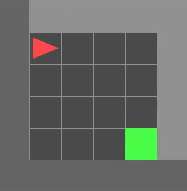
\includegraphics[width=0.7\linewidth]{videos/RLmvs-1.png}}{VPlayer.swf}
        \end{column}
        
    \end{columns}

\begin{columns}<2->
        \begin{column}{0.6\textwidth}
        \small{        
            \begin{itemize}
                \item Sub-optimal trajectory forced with IRL
                \item The user controls the agent behaviour
            \end{itemize}
        }
            
        \end{column}
        \begin{column}{0.4\textwidth}
            \includemedia[width=0.7\linewidth, keepaspectratio, passcontext,
                transparent, addresource=videos/IRLmvs.mp4, noplaybutton,
                flashvars={source=videos/IRLmvs.mp4&autoPlay=true&loop=true}
                ]{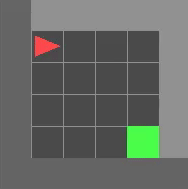
\includegraphics[width=0.7\linewidth]{videos/IRLmvs-1.png}}{VPlayer.swf}
        \end{column}
        
    \end{columns}
    
\end{frame}

% Tuning slide
\begin{frame}{Tuning the components}
    \begin{itemize}
        \item Policy
        \begin{itemize}
            \item the agent has to reach easily the  environment goal $\Rightarrow$ episode length 150
            \item no negative goal reward or big values range $\Rightarrow$ standard deviation 0.5 
        \end{itemize} 

        \vspace{0.2cm}
        \pause
        \item Annotator
        \begin{itemize}
            \item sparse vs dense Oracle
        \end{itemize}
        
        \vspace{0.2cm}
        \pause
        \item Reward Model
        \begin{itemize}
            \item variable K batch vs constant K batch
            \item early stopping and decreasing annotations
        \end{itemize}
    \end{itemize}
\end{frame}

% Reward model loss
\begin{frame}{Reward Model Loss}

    \begin{itemize}
        \item The reward model loss grows during the training protocol.
    \end{itemize}
    \centering
    \vspace{0.4cm}
    \includegraphics<1>[width=0.6\linewidth]{images/reward_loss.png}
    
    
\end{frame}

% Reward model loss
\begin{frame}{}
\centering

\includegraphics[width=1\linewidth]{images/bothlosses.png}

\begin{adjustwidth}{-2em}{-2em}
    \begin{columns}
        \begin{column}{0.5\textwidth}
        \small{        
            \begin{itemize}
                \item Small contribution to total loss
                \item Same range during all the training
            \end{itemize}
        }
            
        \end{column}
        \begin{column}{0.5\textwidth}
        \small{
            \begin{itemize}
                \item Big contribution to total loss
                \item The number of those preferences make the loss grow
            \end{itemize}
        }
        
        \end{column}
        
    \end{columns}
\end{adjustwidth}
\end{frame}

